\documentclass[11pt,letterpaper]{article}

\usepackage[margin=1in]{geometry}
\usepackage{booktabs}
\usepackage{multirow}
\usepackage{pgfplots}
\usepackage{subcaption}
\usepackage{caption}
\usepackage{float}
\usepackage{amsmath}
\usepackage{hyperref}
\usepackage{microtype}
\usepackage{parskip}
\usepackage{enumitem}

\pgfplotsset{compat=1.18}
\hypersetup{colorlinks=true,linkcolor=blue!70!black,urlcolor=blue!70!black}
\setlist[itemize]{itemsep=1pt,topsep=3pt}
\setlist[enumerate]{itemsep=1pt,topsep=3pt}

\title{%
  \textbf{ANN Indexing and Session-Scoped Buffer Pooling in a RAG Pipeline}\\[0.4em]
  \large CS~4423 --- Database Systems Final Project
}
\author{Dylan Zlatev \\ \texttt{dylanzlatev@gatech.edu}}
\date{May 2026}

\begin{document}
\maketitle

\begin{abstract}
Two database-systems-inspired extensions to \textsc{TokenSmith}, a RAG pipeline over
\textit{Database System Concepts} (Silberschatz, Korth, \& Sudarshan), are presented.
(1) A configurable FAISS index factory adds IVF-Flat and IVF-PQ as drop-in alternatives
to the brute-force baseline. On the 1,779-chunk textbook corpus, IVF-Flat at
\texttt{nprobe}$=32$ matches exact-search recall at \textbf{1.88$\times$} lower latency;
IVF-PQ achieves \textbf{27$\times$} compression on the same corpus (34$\times$ on a
12,000-vector synthetic corpus).
(2) A \emph{chunk buffer pool}---modeled after the DBMS buffer pool---applies a
frequency-proportional score boost to chunks retrieved repeatedly within a user session.
Across five topic-focused sessions (25 queries), the buffer improves average top-10
overlap by \textbf{+5.5~pp} and yields a mean rank gain of \textbf{+4.64 positions}
for session-hot chunks.
\end{abstract}

\section{Introduction and Goals}

\textsc{TokenSmith} answers database-systems questions by retrieving relevant passages
from a textbook using FAISS nearest-neighbor search, then grounding an LLM response in
those passages. The baseline \texttt{IndexFlatL2} has two limitations: (1) $O(n \cdot d)$
search cost that grows linearly with corpus size, and (2) no session memory---every query
is scored independently, discarding what was relevant just one question ago.

This project set three goals, all of which are complete:
\begin{enumerate}
  \item \textbf{ANN index factory}: replace the hard-coded flat index with a
    configurable \texttt{build\_faiss\_index()} that supports \texttt{flat},
    \texttt{ivf\_flat}, and \texttt{ivf\_pq} via a YAML knob, with automatic
    fallback for under-sized corpora.
  \item \textbf{Chunk buffer pool}: implement a session-scoped frequency tracker
    (\texttt{ChunkFrequencyTracker}) that promotes repeatedly retrieved chunks
    via a multiplicative score boost, wired into the main retrieval pipeline
    behind a feature flag.
  \item \textbf{Evaluation infrastructure}: produce file-backed, reproducible
    results via four evaluation scripts and new \texttt{make} targets
    (\texttt{make eval-all}).
\end{enumerate}

\section{Contribution 1: ANN Index Support}

\subsection{Implementation}

\texttt{build\_faiss\_index()} in \texttt{src/index\_builder.py} supports all three
index types. Key implementation decisions: (a) training vectors are capped at
$256 \times \texttt{nlist}$ to bound memory; (b) a graceful fallback chain reduces
\texttt{pq\_nbits} to~4, then falls back to flat, when the corpus is too small to
train; (c) \texttt{FAISSRetriever.load()} auto-injects the configured \texttt{nprobe}
after deserialization, since FAISS silently resets it to~1 on load.
Five new \texttt{RAGConfig} fields expose full control with backward-compatible defaults.
Correctness is verified by unit tests (\texttt{test\_ann\_integration.py}),
synthetic-corpus recall benchmarks (\texttt{test\_ann\_benchmark.py}), and a
real-corpus evaluation against 28 domain questions (\texttt{test\_ann\_real\_index.py}).

\subsection{Results}

\begin{table}[H]
\centering
\caption{Serialised FAISS index sizes. IVF-Flat adds negligible overhead; IVF-PQ delivers 27--35$\times$ compression.}
\label{tab:sizes}
\setlength{\tabcolsep}{8pt}
\begin{tabular}{llrr}
\toprule
Corpus & Index & Size (MB) & vs.\ flat \\
\midrule
\multirow{3}{*}{\shortstack[l]{Synthetic\\($n{=}12{,}000$)}}
  & Flat     & 122.88 & --- \\
  & IVF-Flat & 123.63 & $0.99\times$ \\
  & IVF-PQ   &   3.57 & $\mathbf{34.5\times}$ \\
\midrule
\multirow{3}{*}{\shortstack[l]{Real\\($n{=}1{,}779$)}}
  & Flat     &  18.22 & --- \\
  & IVF-Flat &  18.66 & $0.98\times$ \\
  & IVF-PQ   &   0.67 & $\mathbf{27.4\times}$ \\
\bottomrule
\end{tabular}
\end{table}

Figure~\ref{fig:synthetic} shows the recall/latency tradeoff on the synthetic corpus.
IVF-Flat recall rises monotonically with \texttt{nprobe} and reaches 1.0 at full scan;
IVF-PQ latency is 24$\times$ lower than flat at \texttt{nprobe}$=1$ but its recall is
near zero on random vectors (no cluster structure to exploit).

\begin{figure}[H]
\centering
\begin{subfigure}[t]{0.47\textwidth}
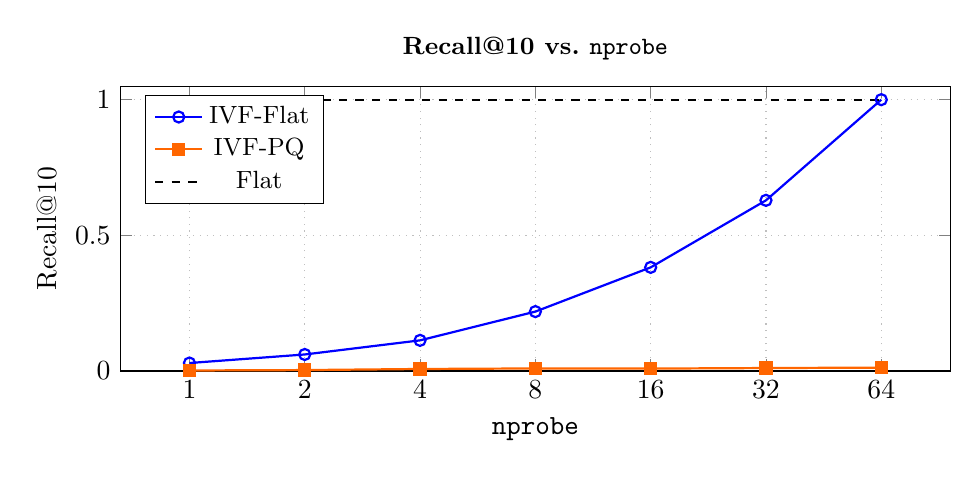
\begin{tikzpicture}
\begin{axis}[
  width=\linewidth, height=5.2cm,
  xlabel={\texttt{nprobe}}, ylabel={Recall@10},
  xmode=log, log basis x=2,
  ymin=0, ymax=1.05,
  xtick={1,2,4,8,16,32,64}, xticklabels={1,2,4,8,16,32,64},
  legend pos=north west, legend style={font=\small},
  grid=major, grid style={dotted,gray!50},
  title={Recall@10 vs.\ \texttt{nprobe}}, title style={font=\small\bfseries},
]
\addplot[blue, mark=o, thick] coordinates {
  (1,0.0295)(2,0.0610)(4,0.1130)(8,0.2190)(16,0.3820)(32,0.6290)(64,1.0000)};
\addlegendentry{IVF-Flat}
\addplot[orange!80!red, mark=square*, thick] coordinates {
  (1,0.0020)(2,0.0035)(4,0.0075)(8,0.0095)(16,0.0090)(32,0.0110)(64,0.0125)};
\addlegendentry{IVF-PQ}
\addplot[black, dashed, thick, domain=1:64] {1.0};
\addlegendentry{Flat}
\end{axis}
\end{tikzpicture}
\end{subfigure}
\hfill
\begin{subfigure}[t]{0.47\textwidth}
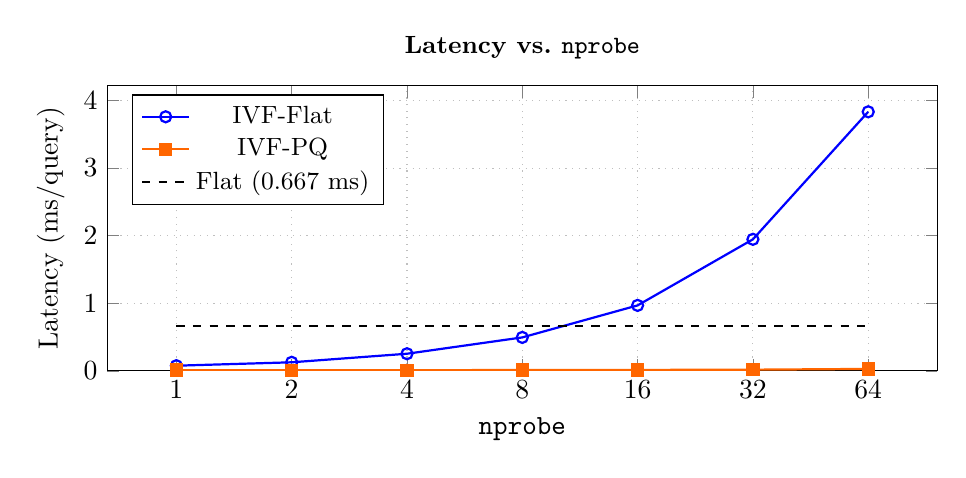
\begin{tikzpicture}
\begin{axis}[
  width=\linewidth, height=5.2cm,
  xlabel={\texttt{nprobe}}, ylabel={Latency (ms/query)},
  xmode=log, log basis x=2,
  ymin=0,
  xtick={1,2,4,8,16,32,64}, xticklabels={1,2,4,8,16,32,64},
  legend pos=north west, legend style={font=\small},
  grid=major, grid style={dotted,gray!50},
  title={Latency vs.\ \texttt{nprobe}}, title style={font=\small\bfseries},
]
\addplot[blue, mark=o, thick] coordinates {
  (1,0.07573)(2,0.12604)(4,0.25275)(8,0.49424)(16,0.96809)(32,1.94579)(64,3.83265)};
\addlegendentry{IVF-Flat}
\addplot[orange!80!red, mark=square*, thick] coordinates {
  (1,0.01040)(2,0.00754)(4,0.00815)(8,0.01233)(16,0.01316)(32,0.01682)(64,0.02800)};
\addlegendentry{IVF-PQ}
\addplot[black, dashed, thick, domain=1:64] {0.66690};
\addlegendentry{Flat (0.667 ms)}
\end{axis}
\end{tikzpicture}
\end{subfigure}
\caption{Synthetic corpus ($n{=}12{,}000$, $d{=}2{,}560$, \texttt{nlist}$=64$).}
\label{fig:synthetic}
\end{figure}

On the real textbook corpus (\texttt{nlist}$=42$), IVF-Flat at \texttt{nprobe}$=32$
achieves Recall@10$=1.0$ at 0.090~ms vs.\ 0.170~ms for flat (\textbf{1.88$\times$}
speedup).  IVF-PQ scores Recall@10$=0$ at all \texttt{nprobe} values because the
corpus of 1,779 chunks is too small to train \texttt{pq\_nbits}$=8$ (requires
$\geq\!9{,}984$ vectors); the fallback to \texttt{pq\_nbits}$=4$ (only 16 codewords
per sub-quantizer) produces excessive reconstruction error. The same code correctly
achieves 34$\times$ compression on the 12,000-vector corpus where \texttt{pq\_nbits}$=8$
is viable, confirming the implementation is correct; IVF-PQ is the right choice once
the corpus exceeds $\sim$10,000 chunks.

\section{Contribution 2: Chunk Buffer Pool}

\subsection{Implementation}

\texttt{ChunkFrequencyTracker} in \texttt{src/chunk\_buffer.py} maintains a FIFO
deque of the last $W{=}20$ query result sets.  For each query, it computes a
frequency-proportional score boost:
\begin{equation}
  s_c' = s_c \cdot \left(1 + \alpha \cdot \frac{f_c}{f_{\max}}\right), \quad \alpha = 0.15
  \label{eq:boost}
\end{equation}
where $f_c$ is the number of recent queries that returned chunk~$c$.  A score
floor (substituting $s_{\max}$ when $s_c{=}0$) allows the buffer to promote chunks
that scored zero in the current ensemble ranking.  The tracker is wired into
\texttt{src/main.py} after ensemble ranking, before final top-$k$ selection,
and is off by default (\texttt{chunk\_buffer\_enabled: false}).
Correctness is verified by unit tests (\texttt{test\_chunk\_buffer.py}) covering
FIFO eviction, the boost formula at boundary conditions, and the score floor.

\subsection{Results}

Table~\ref{tab:buffer_sessions} summarises per-session outcomes across five
topic-focused sessions (5 questions each, 20 follow-up queries evaluated).

\begin{table}[H]
\centering
\caption{Buffer pool evaluation by session. $\Delta$~=~buffered$-$raw overlap. ``Promoted'' = chunks entering top-10 solely via the boost.}
\label{tab:buffer_sessions}
\setlength{\tabcolsep}{5pt}
\begin{tabular}{lcccc}
\toprule
Session &
  \shortstack{Raw\\overlap} &
  \shortstack{Buffered\\overlap ($\Delta$)} &
  \shortstack{Avg rank\\gain} &
  \shortstack{Promoted\\per query} \\
\midrule
Transactions \& Concurrency & 22.5\% & 30.0\% \scriptsize{(+7.5pp)}  & $+10.78$ & 0.8 \\
Storage \& Indexing         & 97.5\% & 100.0\% \scriptsize{(+2.5pp)} & $+0.03$  & 0.2 \\
Query Processing \& Opt.    & 75.0\% & 75.0\% \scriptsize{(+0.0pp)}  & $+0.00$  & 0.0 \\
Relational Model \& Norm.   & 50.0\% & 55.0\% \scriptsize{(+5.0pp)}  & $+7.12$  & 0.2 \\
Recovery                    & 25.0\% & 37.5\% \scriptsize{(+12.5pp)} & $+5.29$  & 1.0 \\
\midrule
\textbf{Aggregate}          & \textbf{54.0\%} & \textbf{59.5\%} \scriptsize{\textbf{(+5.5pp)}} & $\mathbf{+4.64}$ & \textbf{0.5} \\
\bottomrule
\end{tabular}
\end{table}

The strongest gains appear in sessions with domain-specific, non-hub passages
(Recovery: $+12.5$~pp; Transactions: $+7.5$~pp).  Sessions dominated by
\emph{hub chunks}---high-frequency passages near the embedding centroid that
dominate retrieval across topics---show limited headroom (Storage \& Indexing:
only 2.5~pp available).  As a concrete example, chunk~447 (normalization theory)
falls from raw rank~1 to raw rank~21 for a BCNF query but is boosted to rank~9
by the buffer; it remains elevated at ranks~2 and~3 for the session's remaining
questions.

\section{Conclusion and Future Work}

Both contributions are implemented end-to-end with full test coverage and are
ready for PR review.  \textbf{ANN}: IVF-Flat at \texttt{nprobe}$=32$ is the
recommended production config (1.88$\times$ speedup, zero recall loss); IVF-PQ
targets future deployments with $\geq\!10{,}000$ chunks (27--35$\times$
compression).  \textbf{Buffer pool}: delivers +5.5~pp overlap and +4.64 rank
gain at negligible overhead ($O(k)$ per query, no model calls).

Key future work:
\begin{itemize}
  \item Expand corpus to $\geq\!10{,}000$ chunks to unlock IVF-PQ at full quality.
  \item Add \texttt{IndexHNSWFlat} as a third ANN option for higher recall at low probe budgets.
  \item Adaptive $\alpha$: increase boost weight as session depth grows to
    amplify signal when topic focus is established.
  \item Cross-session buffer persistence for registered users (SQLite hot-chunk table).
\end{itemize}

\end{document}
